\section{Discussion}
\label{sec:discussion}

\begin{figure*}
\vskip-5mm
\begin{center}
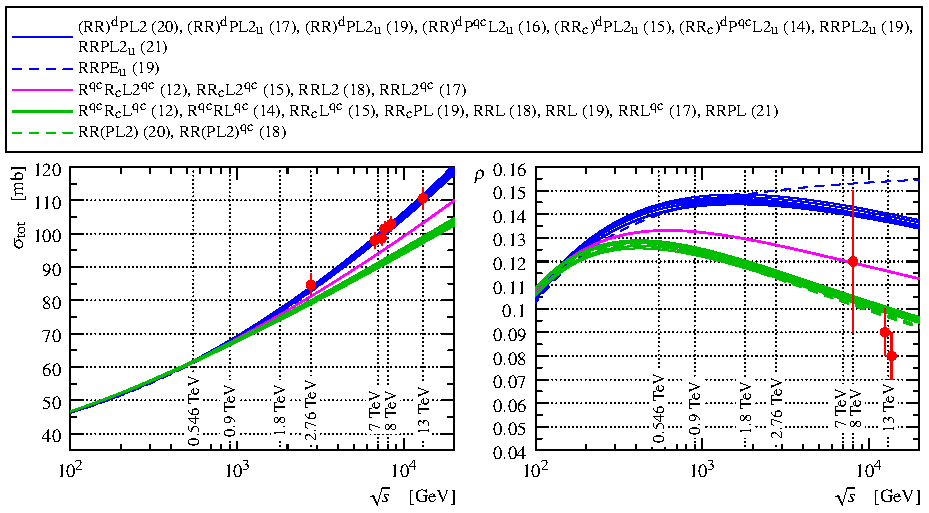
\includegraphics{fig/compete_bands_si_tot_rho.pdf}
\caption{%
Predictions of COMPETE models \cite{compete-details} for $\rm pp$ interactions. Each model is represented by a line (see legend). The red points represent the reference TOTEM measurements. \TODO{add sigma tot determination from this publication ?}
}
\label{fig:comp bands}
\end{center}
\end{figure*}

On of very comprehensive (and therefore representative) studies of the pre-LHC data is by the COMPETE collaboration \cite{compete}. In total 256 models have been considered to describe $\sigma_{\rm tot}$ and $\rho$ data for various reactions ($\rm pp$, $\rm p\pi$, $\rm pK$, etc.) and their anti-reactions. Out of these models, 23 have been found to give reasonable description of the data \cite{compete-details}. These models are confronted with newer TOTEM data in Figure~\ref{fig:comp bands}, showing that the COMPETE models form 3 bands plotted in different colours. The blue band is well compatible (p-value $0.99$) with the $\sigma_{\rm tot}$ data, but incompatible (p-value $2\cdot10^{-4}$) with $13\un{TeV}$ $\rho$ point. The magenta band is incompatible (p-value $4\cdot10^{-5}$) with the $\sigma_{\rm tot}$ data and at the limit of compatibility (p-value $0.11$) with the $\rho$ point. The green band is incompatible (p-value $2\cdot10^{-16}$) with the $\sigma_{\rm tot}$ data, but compatible (p-value $0.84$) with the $\rho$ point. For the evaluation of the p-values, the measurements were considered as independent which can be justified by using data from different LHC fills, using different beam optics, often different energies, often using different RPs, often different analysis approaches (fit parametrisation, treatment of CNI) and often analysed by different teams. In summary, none of the COMPETE models is compatible with the ensemble of TOTEM's $\sigma_{\rm tot}$ and $\rho$ measurements.

Another, even less model-dependent, relation between $\sigma_{\rm tot}$ and $\rho$ can be obtained from dispersion relations \TODO{reference}. If only cross-even component of the amplitude is considered, it can be shown that $\rho$ is proportional to the rate of growth of $\sigma_{\rm tot}$ with energy. This again presents a contradiction to the presented data featuring sustained growth of $\sigma_{\rm tot}$ while low value of $\rho$.

The above observations seem to suggest a need for a crossing-odd component in the amplitude. While at lower energies such contributions may naturally come from secondary Reggeons \TODO{examples}, their contribution is generally considered negligible at LHC energies due to their intercept lower than unity.

A variety of such crossing-odd components have been discussed in literature, within different frameworks and under different names. The ``Odderon'' was proposed within the axiomatic theory \cite{nicolescu-1990,nicolescu-2007} as an amplitude contribution responsible for $\sigma_{\rm tot}^{\rm p\bar p} - \sigma_{\rm tot}^{\rm pp} \propto \log s$ and also for the $\rm p\bar p$ and $\rm pp$ difference of the differential cross-section in the dip region. The Odderon was also studied within the Regge theory as the crossing-odd counterpart of the Pomeron \TODO{reference}. It has also been shown that such object must exist in QCD, as a colourless bound state of three gluons with quantum numbers $J^{PC} = 1^{--}$ \TODO{reference}. These 3 gluons are bound together more strongly than their interaction with other particle is. There is also evidence for such state in QCD lattice calculations, known under names ``oddball'' or ``vector glueball'' \TODO{reference}. Such a state can be exchanged in $t$-channel and contribute, e.g., to the elastic amplitude, as well as can be created in the $s$-channel and thus be observed in spectroscopic studies. More details can be found in reviews \cite{braun,ewerz}.

There are multiple ways how such a crossing-odd component may manifest in observable data. Focusing on elastic scattering at the LHC (unpolarised beams), there are 3 regions argued to be sensitive. In general, the effects of Odderon are expected to be much smaller than those of the Pomeron. Consequently, the sensitive regions are those where the Pomeron contributions cancel or are limited in size. At very low $|t|$ the Pomeron amplitude is expected almost purely imaginary, while the Odderon would make contributions to the real part and therefore $\rho$ is a very sensitive parameter. Another such example is the dip, often described by the imaginary part of the amplitude crossing zero, thus making visible the real part to which Odderon may contribute. In agreement with such predictions, the observed dips in $\rm p\bar p$ scattering tend to be shallower than those in $\rm pp$. At $\sqrt s \approx 62\un{GeV}$, there are data showing very significant difference between the $\rm pp$ and $\rm p\bar p$ dip. The interpretation of this difference is, however, complicated due to non-negligible contribution from secondary Reggeons. This dip difference is also predicted to be energy-dependent which presents another experimental observable. Sometimes high $|t|$ region is also argued as sensitive to the Odderon since the Pomeron contribution is rapidly dropping. However, preliminary high-$|t|$ TOTEM data at $13\un{TeV}$ indicate that this region is dominated by yet another pQCD amplitude.

Figure~\ref{fig:match models} shows two models that are compatible with TOTEM data: by Nicolescu et al.~\cite{nicolescu-2017} and the Durham model \cite{durham-2017-note}. In both cases, inclusion of the cross-odd component leads to an improvement of the agreement between the data and model. While for the Nicolescu model the Odderon effect is large and strongly energy-dependent, for the Durham model the effect is smaller and relatively flat in energy.

\begin{figure*}
\vskip-5mm
\begin{center}
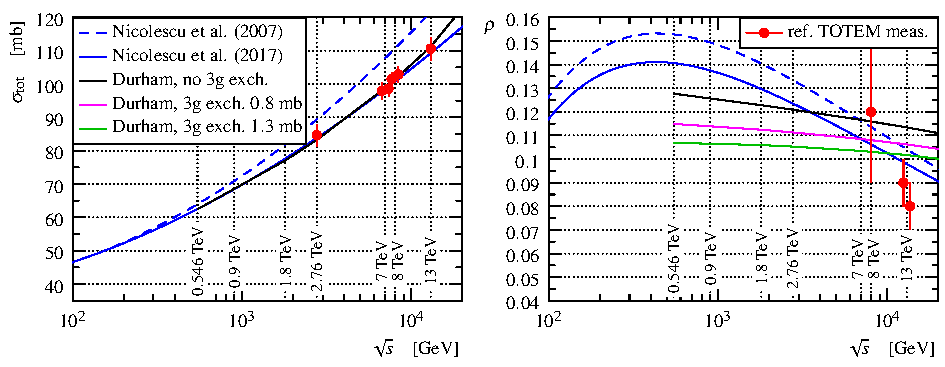
\includegraphics{fig/matching_models_si_tot_rho.pdf}
\caption{%
Predictions of the model by Nicolescu et al.~\cite{nicolescu-2017} (blue) and the Durham model \cite{durham-2017-note} (green) compared to the reference TOTEM measurements (red). \TODO{keep only one curve from Durham}
}
\label{fig:match models}
\end{center}
\end{figure*}
